\chapter{ゼロから始める(開発環境構築)}
\label{chap:01-createDevEnv}
\begin{reviewimage}%%01_00asignToFrontend
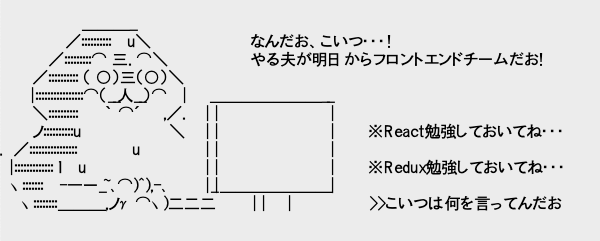
\includegraphics[width=1.0\maxwidth]{./images/01-createDevEnv/01_00asignToFrontend.png}%
\reviewimagecaption{やる夫が、突然の移動を命じられたお!}
\label{image:01-createDevEnv:01_00asignToFrontend}
\end{reviewimage}
\begin{starterabstract}
  本章では、React、Reduxの開発環境を作成します。\\[0pt]

「なぜ、これらが必要なのか?」\\[0pt]

  は、とりあえず置いといて\\[0pt]
   ・ Node.js\\[0pt]
   ・ Microsoft Visual Studio Code + 拡張機能\\[0pt]
   ・ Google Chrome + 拡張機能\\[0pt]
をインストールしてください。これらは、すべて無償で提供されています。\\[0pt]
\\[0pt]
なお、これらの準備が整っている方は、本章を読み飛ばしていただいてもかまいません。
\end{starterabstract}

\section{ Node.js}
\keeplastskip{
  \label{sec:1-1}
  \label{sec-nodejs}
  \par\nobreak
}

\subsection{Node.jsについて}
\keeplastskip{
  \label{sec:1-1-1}
  \par\nobreak
}

\subsubsection*{Node.jsとは?}
\keeplastskip{
  \label{sec:1-1-1-1}
  \par\nobreak
}

「Node.js」は、通常ブラウザ上で実行されるJavaScriptをサーバやPC上で実行できるようする
「{\reviewstrong{JavaScript実行環境}}」です。
たとえば、WindowsにPythonをインストールすると「python.exe」を使いpythonファイルをWindows上で実行できます。

\begin{reviewimage}%%y01
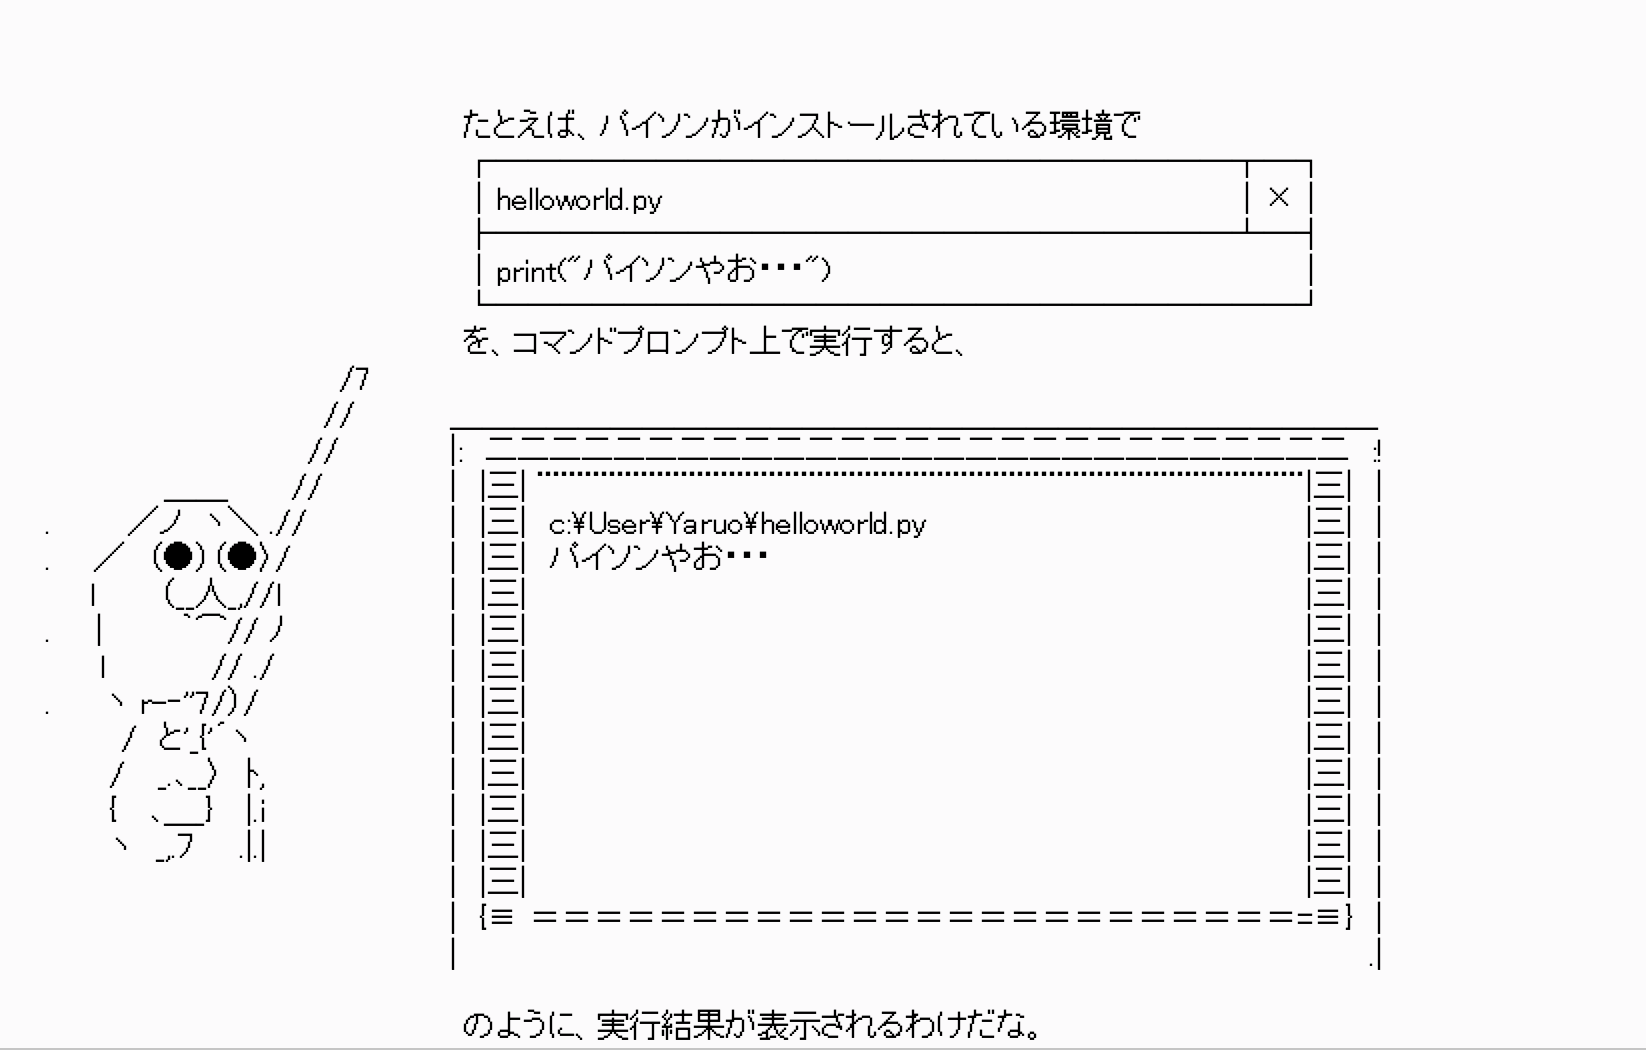
\includegraphics[width=1.0\maxwidth]{./images/01-createDevEnv/y01.png}%
\reviewimagecaption{pythonを実行}
\label{image:01-createDevEnv:y01}
\end{reviewimage}

同じように、{\reviewstrong{Node.js}}をインストールすると、「node.exe」を使いJavaScriptファイルを実行できます。
たとえば、以下のように「test01.js」ファイルを作成します。

\def\startercodeblockfontsize{}
\begin{starterprogram}[test01.js]{リスト1.1: }\seqsplit{  const name='やる夫';
  const message='こまけぇこたぁいいんだよ';

  console.log(`\textdollar{}\{name\}が、こんなこと言ってます。\textdollar{}\{message\}`);}\end{starterprogram}

このスクリプトをターミナル上で実行します。「node」コマンドに実行したいJavaScriptファイルを引数として渡します。

\def\startercodeblockfontsize{}
\begin{starterterminal}[_152393477]{リスト1.2: app.jsを実行}\seqsplit{  ❯ node test01.js
  やる夫が、こんなこと言ってます。こまけぇこたぁいいんだよ}\end{starterterminal}

このように、今まではJavaScriptの実行環境はブラウザでしたが、NodeがあればJacaScriptをPC、サーバで実行できます。


\clearpage


\subsubsection*{Node.jsについて}
\keeplastskip{
  \label{sec:1-1-1-2}
  \par\nobreak
}
\begin{reviewimage}%%y01_getNodejs
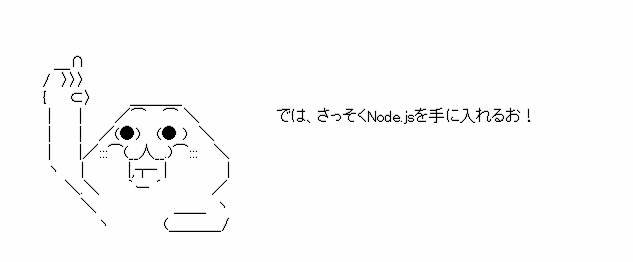
\includegraphics[width=1.0\maxwidth]{./images/01-createDevEnv/y01_getNodejs.png}%
\reviewimagecaption{Node.jsをインストールするお!}
\label{image:01-createDevEnv:y01_getNodejs}
\end{reviewimage}
\begin{reviewimage}%%yr01_aboutNodejs
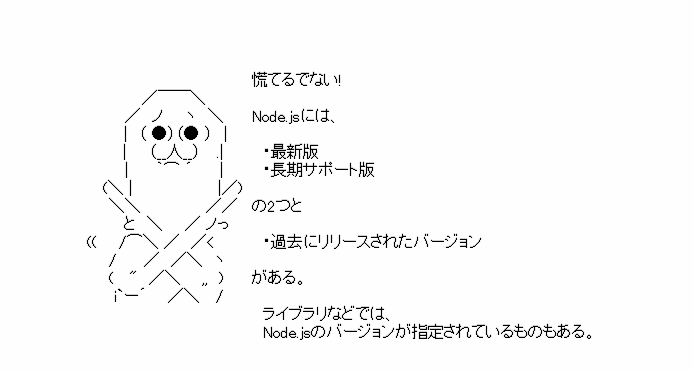
\includegraphics[width=1.0\maxwidth]{./images/01-createDevEnv/yr01_aboutNodejs.png}%
\reviewimagecaption{Node.jsのバージョンには注意}
\label{image:01-createDevEnv:yr01_aboutNodejs}
\end{reviewimage}

では、Node.jsの本家トップページ:\url{https://nodejs.org/ja/}へアクセスします。

\begin{reviewimage}[H]%%01_01nodejsTop
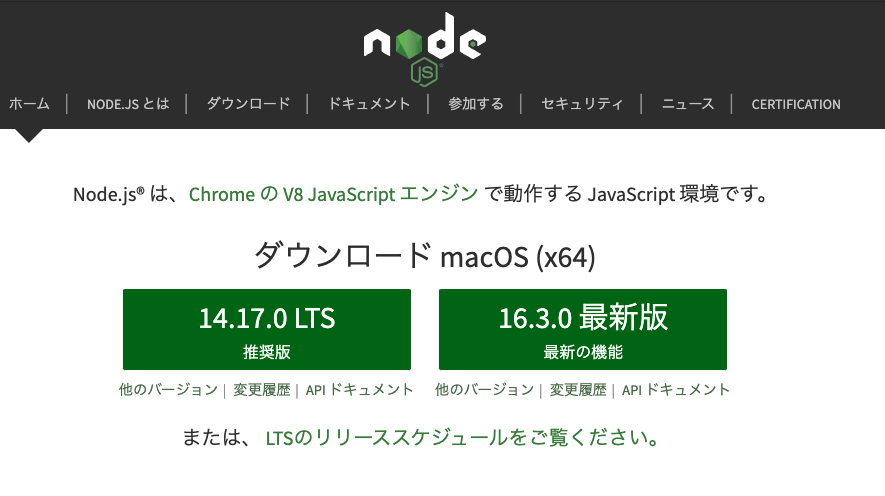
\includegraphics[width=1.0\maxwidth]{./images/01-createDevEnv/01_01nodejsTop.png}%
\reviewimagecaption{Node.jsトップページ}
\label{image:01-createDevEnv:01_01nodejsTop}
\end{reviewimage}

ここでダウンロード可能なのは、「16.13.1 LTS(Long Term Support)推奨版」と「17.3.0最新版」\footnote{2022/12/17現在}の2つがあります。

LTS版、最新版は以下のロードマップにより更新されます。

\begin{reviewimage}[H]%%01_02nodejsRoadmap
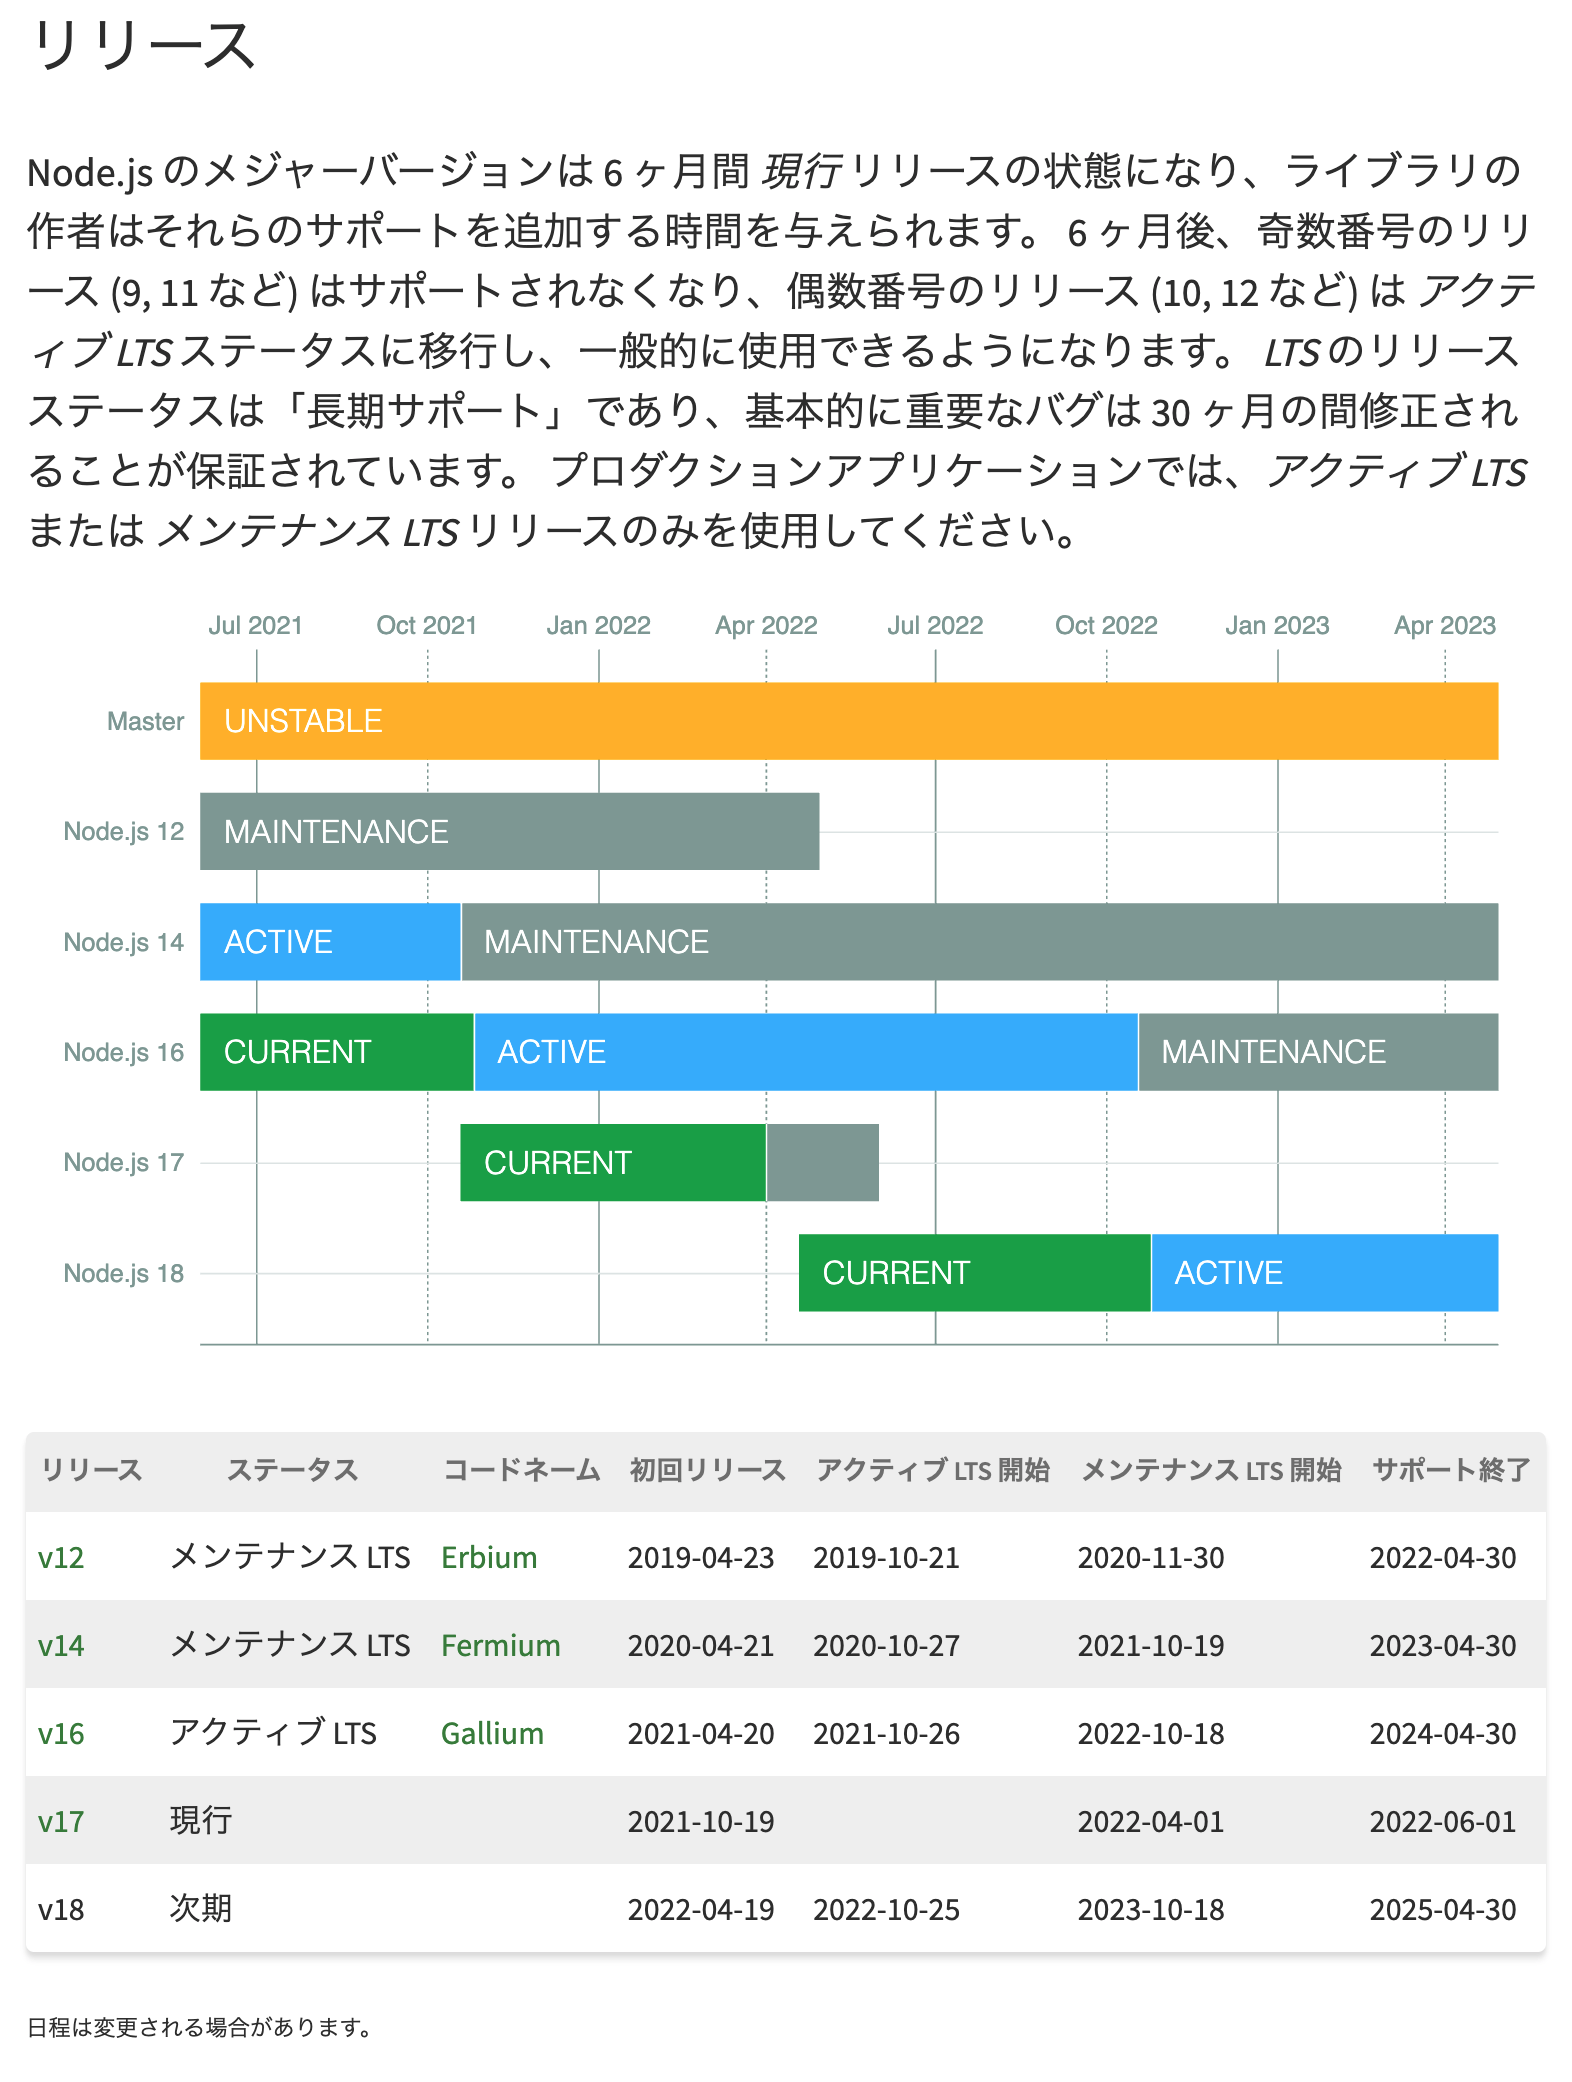
\includegraphics[width=1.0\maxwidth]{./images/01-createDevEnv/01_02nodejsRoadmap.png}%
\reviewimagecaption{Node.jsロードマップ}
\label{image:01-createDevEnv:01_02nodejsRoadmap}
\end{reviewimage}

\clearpage


Node.jsのReleases:\url{https://nodejs.org/ja/about/releases/}にあるように、
Node.jsは、各年の4月、10月にリリースされ、

\begin{starteritemize}
\item Current
\item Active
\item Maintenance
\end{starteritemize}

のフェーズを経ますが、メジャーバージョン番号が偶数のものだけが、Active期間を経て長期サポートされます。

\vspace*{\baselineskip}

上記トップページにあるNode.js 16は、2024/4/30までの長期サポートとなります。
実際のプロジェクトで使用する場合は、よほどの理由がない限りは最新のLTS版を使用します。

\subsection{Node.jsのインストールの前に}
\keeplastskip{
  \label{sec:1-1-2}
  \par\nobreak
}
\begin{reviewimage}%%y01_whichNodeVer
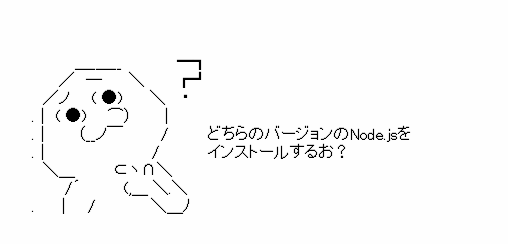
\includegraphics[width=1.0\maxwidth]{./images/01-createDevEnv/y01_whichNodeVer.png}%
\label{image:01-createDevEnv:y01_whichNodeVer}
\end{reviewimage}

Node.jsは、ロードマップにより定期的にバージョンアップされます。又、Node.js自体の不具合の修正などで
マイナーバージョンアップも行われます。

\vspace*{\baselineskip}

プロジェクト開発中のマイナーバージョンアップでも検証が必要になりますが、
メジャーバージョンアップの場合はさらに大きな検証が必要になります。
場合によっては、ソースコードの大幅な改良をしなければならなくなります。

\vspace*{\baselineskip}

それを避けるためにも、プロジェクト毎にNode.jsのバージョンは固定して開発します。

\vspace*{\baselineskip}

通常は、OSにインストールできるNode.jsのバージョンはひとつですが、長期にわたるサポートや新規プロジェクト開発のためには、
複数のNode.jsのバージョンを切り替えて使用できるしくみを用意しましょう。

\vspace*{\baselineskip}

私が使用しているのは、nvm(node version manager):\url{https://github.com/nvm-sh/nvm}です。
いろいろなバージョンのNode.jsを、簡単にインストール・アンインストール・切替ができます。

\vspace*{\baselineskip}

「nvm」も含めたNode.jsバージョン管理ツールについては、
こちらの@heppokofrontendさんの良記事が参考になります。

\begin{reviewimage}%%01_nodeVersionChange
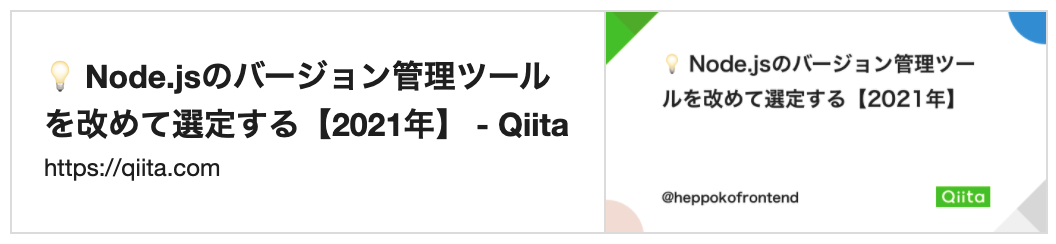
\includegraphics[width=1.0\maxwidth]{./images/01-createDevEnv/01_nodeVersionChange.png}%
\label{image:01-createDevEnv:01_nodeVersionChange}
\end{reviewimage}

Node.jsのバージョン管理ツールを改めて選定する【2021年】\footnote{\url{https://qiita.com/heppokofrontend/items/5c4cc738c5239f4afe02}}

\subsection{nvm}
\keeplastskip{
  \label{sec:1-1-3}
  \par\nobreak
}

nvm(node version manager)を使えば、複数バージョンのNode.jsを1台のPCにインストールし、バージョンを切り替えることが簡単にできます。

\vspace*{\baselineskip}

GitHub上のnvmは、Shellscript(sh, dash, zsh, bash)上で動作するため、Linux(UNIX系)、macOSにインストールできます。

\vspace*{\baselineskip}

Windows版:\url{https://github.com/coreybutler/nvm-windows}は、別な方がGitHub上で公開されています。
コマンドが本家と少し違いますが、複数バージョンのインストール・バージョンの切り替えなど機能は問題ありません。

\paragraph*{nvmのインストール}
\paragraph*{macOS}
お使いのTerminalから以下のコマンドを実行してください。

\def\startercodeblockfontsize{}
\begin{starterterminal}[_120372761]{リスト1.3: nvmのインストール}\seqsplit{  \textgreater{}curl {-}o{-} https://raw.githubusercontent.com/nvm{-}sh/nvm/v0.39.0/install.sh \textbar{} bash}\end{starterterminal}

インストール完了後には、.zshrcへ以下を追加してください。

\def\startercodeblockfontsize{}
\begin{starterterminal}[]{.zshrcへ追加}\seqsplit{  export NVM\textunderscore{}DIR="\textdollar{}([ {-}z "\textdollar{}\{XDG\textunderscore{}CONFIG\textunderscore{}HOME{-}\}" ] \&\& printf \%s "\textdollar{}\{HOME\}/.nvm" \textbar{}\textbar{} printf \%s "\textdollar{}\{XDG\textunderscore{}CONFIG\textunderscore{}HOME\}/nvm")"
[ {-}s "\textdollar{}NVM\textunderscore{}DIR/nvm.sh" ] \&\& \reviewbackslash{}. "\textdollar{}NVM\textunderscore{}DIR/nvm.sh" \# This loads nvm}\end{starterterminal}
\ParagraphEnd

\paragraph*{Windows}
nvm{-}windowsのリリースページ:\url{https://github.com/coreybutler/nvm-windows/releases/tag/1.1.8}より、
最新版をダウンロードしインストールしてください。

\ParagraphEnd

\subsubsection*{nvmの使い方}
\keeplastskip{
  \label{sec:1-1-3-1}
  \par\nobreak
}

macOSではターミナルを起動し、Windowsではコマンドプロンプト、または、Windows Terminalを起動してください。

nvmとnvm{-}windowsでは、コマンドが少し違いますが、「nvm {-}{-}help」を入力することで使用できるコマンドが表示されます。

\def\startercodeblockfontsize{}
\begin{starterterminal}[]{Mac OSX}\seqsplit{\textgreater{} nvm {-}{-}help

Node Version Manager (v0.37.2)
{\reviewballoon{中略}}
Example:
  nvm install 8.0.0                     Install a specific version number
  nvm use 8.0                           Use the latest available 8.0.x release
  nvm run 6.10.3 app.js                 Run app.js using node 6.10.3
  nvm exec 4.8.3 node app.js            Run `node app.js` with the PATH pointing to node 4.8.3
  nvm alias default 8.1.0               Set default node version on a shell
  nvm alias default node                Always default to the latest available node version on a shell

{\reviewballoon{中略}}
Note:
  to remove, delete, or uninstall nvm {-} just remove the `\textdollar{}NVM\textunderscore{}DIR` folder (usually `\textasciitilde{}/.nvm`)}\end{starterterminal}

もし、32bit版Windowsをお使いの場合には、インストールの際に32bit版を指定する「32」をコマンドの最後につけてください。

\def\startercodeblockfontsize{}
\begin{starterterminal}[]{windows}\seqsplit{PS C:\reviewbackslash{}Users\reviewbackslash{}inabakazuya\textgreater{} nvm {-}{-}help

Running version 1.1.7.

Usage:

  nvm arch                     : Show if node is running in 32 or 64 bit mode.
  nvm install \textless{}version\textgreater{} [arch] : The version can be a Node.js version or "latest" for the latest stable version.
                                 Optionally specify whether to install the 32 or 64 bit version (defaults to system arch).
                                 Set [arch] to "all" to install 32 AND 64 bit versions.
                                 Add {-}{-}insecure to the end of this command to bypass SSL validation of the remote download server.
  nvm list [available]         : List the Node.js installations. Type "available" at the end to see what can be installed. Aliased as ls.
{\reviewballoon{中略}}
  nvm uninstall \textless{}version\textgreater{}      : The version must be a specific version.
  nvm use [version] [arch]     : Switch to use the specified version. Optionally specify 32/64bit architecture.
                                 nvm use \textless{}arch\textgreater{} will continue using the selected version, but switch to 32/64 bit mode.
  nvm root [path]              : Set the directory where nvm should store different versions of Node.js.
                                 If \textless{}path\textgreater{} is not set, the current root will be displayed.
  nvm version                  : Displays the current running version of nvm for Windows. Aliased as v.}\end{starterterminal}
\ParagraphEnd

\paragraph*{インストール可能なNode.jsを表示\\[0pt]}
まずは、インストール可能なNode.jsのバージョンを表示してみます。
macOSの場合には、古いバージョンから最新バージョンまでが表示されます。

\def\startercodeblockfontsize{}
\begin{starterterminal}[]{Mac OSX}\seqsplit{\textgreater{}nvm ls{-}remote
{\reviewballoon{古いバージョンから全て表示されるので中略}}
v14.13.1
v14.14.0
v14.15.0   (LTS: Fermium)
v14.15.1   (LTS: Fermium)
v14.15.2   (Latest LTS: Fermium)
 v15.0.0
 v15.0.1
 v15.1.0
 v15.2.0
 v15.2.1
 v15.3.0
 v15.4.0}\end{starterterminal}

\clearpage


一方、Windowsの場合には、表形式で表示されます。新しいバージョンが上に表示されます。

\def\startercodeblockfontsize{}
\begin{starterterminal}[]{Windows}\seqsplit{PS C:\reviewbackslash{}Users\reviewbackslash{}inabakazuya\textgreater{} nvm list available

\textbar{}   CURRENT    \textbar{}     LTS      \textbar{}  OLD STABLE  \textbar{} OLD UNSTABLE \textbar{}
\textbar{}{-}{-}{-}{-}{-}{-}{-}{-}{-}{-}{-}{-}{-}{-}\textbar{}{-}{-}{-}{-}{-}{-}{-}{-}{-}{-}{-}{-}{-}{-}\textbar{}{-}{-}{-}{-}{-}{-}{-}{-}{-}{-}{-}{-}{-}{-}\textbar{}{-}{-}{-}{-}{-}{-}{-}{-}{-}{-}{-}{-}{-}{-}\textbar{}
\textbar{}    15.4.0    \textbar{}   14.15.2    \textbar{}   0.12.18    \textbar{}   0.11.16    \textbar{}
\textbar{}    15.3.0    \textbar{}   14.15.1    \textbar{}   0.12.17    \textbar{}   0.11.15    \textbar{}
\textbar{}    15.2.1    \textbar{}   14.15.0    \textbar{}   0.12.16    \textbar{}   0.11.14    \textbar{}
\textbar{}    15.2.0    \textbar{}   12.20.0    \textbar{}   0.12.15    \textbar{}   0.11.13    \textbar{}
\textbar{}    15.1.0    \textbar{}   12.19.1    \textbar{}   0.12.14    \textbar{}   0.11.12    \textbar{}
\textbar{}    15.0.1    \textbar{}   12.19.0    \textbar{}   0.12.13    \textbar{}   0.11.11    \textbar{}
\textbar{}    15.0.0    \textbar{}   12.18.4    \textbar{}   0.12.12    \textbar{}   0.11.10    \textbar{}
\textbar{}   14.14.0    \textbar{}   12.18.3    \textbar{}   0.12.11    \textbar{}    0.11.9    \textbar{}
\textbar{}   14.13.1    \textbar{}   12.18.2    \textbar{}   0.12.10    \textbar{}    0.11.8    \textbar{}
\textbar{}   14.13.0    \textbar{}   12.18.1    \textbar{}    0.12.9    \textbar{}    0.11.7    \textbar{}
\textbar{}   14.12.0    \textbar{}   12.18.0    \textbar{}    0.12.8    \textbar{}    0.11.6    \textbar{}
\textbar{}   14.11.0    \textbar{}   12.17.0    \textbar{}    0.12.7    \textbar{}    0.11.5    \textbar{}
\textbar{}   14.10.1    \textbar{}   12.16.3    \textbar{}    0.12.6    \textbar{}    0.11.4    \textbar{}
\textbar{}   14.10.0    \textbar{}   12.16.2    \textbar{}    0.12.5    \textbar{}    0.11.3    \textbar{}
\textbar{}    14.9.0    \textbar{}   12.16.1    \textbar{}    0.12.4    \textbar{}    0.11.2    \textbar{}
\textbar{}    14.8.0    \textbar{}   12.16.0    \textbar{}    0.12.3    \textbar{}    0.11.1    \textbar{}
\textbar{}    14.7.0    \textbar{}   12.15.0    \textbar{}    0.12.2    \textbar{}    0.11.0    \textbar{}
\textbar{}    14.6.0    \textbar{}   12.14.1    \textbar{}    0.12.1    \textbar{}    0.9.12    \textbar{}
\textbar{}    14.5.0    \textbar{}   12.14.0    \textbar{}    0.12.0    \textbar{}    0.9.11    \textbar{}
\textbar{}    14.4.0    \textbar{}   12.13.1    \textbar{}   0.10.48    \textbar{}    0.9.10    \textbar{}

This is a partial list. For a complete list, visit https://nodejs.org/download/release}\end{starterterminal}
\ParagraphEnd

\paragraph*{Node.js 最新LTS版をインストール}
それでは、最新のLTS版をインストールします。
インストールは、Mac、Windowsとも、「nvm install xx.yy.zz(インストールするバージョン番号)」でインストールできます。

\def\startercodeblockfontsize{}
\begin{starterterminal}[]{Mac OSX}\seqsplit{\textgreater{} nvm install v14.15.2
Downloading and installing node v14.15.2...
Downloading https://nodejs.org/dist/v14.15.2/node{-}v14.15.2{-}darwin{-}x64.tar.xz...
\#\#\#\#\#\#\#\#\#\#\#\#\#\#\#\#\#\#\#\#\#\#\#\#\#\#\#\#\#\#\#\#\#\#\#\#\#\#\#\#\#\#\#\#\#\#\#\#\#\#\#\#\#\#\#\#\#\#\#\#\#\#\#\#\#\#\#\#\#\#\#\#\#\#\#\#\#\#\#\#\#\#\#\#\#\#\#\#\#\#\#\#\#\#\#\#\#\#\#\#\#\#\#\#\#\#\#\#\#\#\#\#\# 100.0\%
Computing checksum with shasum {-}a 256
Checksums matched!
Now using node v14.15.2 (npm v6.14.9)}\end{starterterminal}
\def\startercodeblockfontsize{}
\begin{starterterminal}[]{Window}\seqsplit{PS C:\reviewbackslash{}Users\reviewbackslash{}inabakazuya\textgreater{} nvm install v14.15.2
Downloading Node.js version 14.15.2 (64{-}bit)...
Complete
Creating C:\reviewbackslash{}Users\reviewbackslash{}inabakazuya\reviewbackslash{}AppData\reviewbackslash{}Roaming\reviewbackslash{}nvm\reviewbackslash{}temp

Downloading npm version 6.14.9... Complete
Installing npm v6.14.9...

Installation complete. If you want to use this version, type

nvm use 14.15.2}\end{starterterminal}

\paragraph*{インストールされているNode.jsのバージョンの確認}
インストールされているNode.jsのバージョンは、「nvm ls」で表示させ確認できます。

\def\startercodeblockfontsize{}
\begin{starterterminal}[]{Mac OSX}\seqsplit{\textdollar{} \textgreater{} nvm ls
          v8.17.0
         v12.19.0
         v14.15.0
  {-}\textgreater{}     v14.15.2
           system
  default {-}\textgreater{} v12.18.3
  iojs {-}\textgreater{} N/A (default)
  unstable {-}\textgreater{} N/A (default)
  node {-}\textgreater{} stable ({-}\textgreater{} v14.15.2) (default)
  stable {-}\textgreater{} 14.15 ({-}\textgreater{} v14.15.2) (default)
  lts/* {-}\textgreater{} lts/fermium ({-}\textgreater{} v14.15.2)
  lts/argon {-}\textgreater{} v4.9.1 ({-}\textgreater{} N/A)
  lts/boron {-}\textgreater{} v6.17.1 ({-}\textgreater{} N/A)
  lts/carbon {-}\textgreater{} v8.17.0
  lts/dubnium {-}\textgreater{} v10.23.0 ({-}\textgreater{} N/A)
  lts/erbium {-}\textgreater{} v12.20.0 ({-}\textgreater{} N/A)
  lts/fermium {-}\textgreater{} v14.15.2}\end{starterterminal}
\def\startercodeblockfontsize{}
\begin{starterterminal}[]{Windows}\seqsplit{PS C:\reviewbackslash{}Users\reviewbackslash{}inabakazuya\textgreater{} nvm ls

    14.15.2
    14.15.1
    12.13.1
  * 8.16.1 (Currently using 64{-}bit executable)}\end{starterterminal}

\paragraph*{使用するNode.jsのバージョン切り替え}
先ほどの「インストールされているNode.jsのバージョン表示」で、現在使われているNode.jsのバージョンも表示されています。
使用するNode.jsのバージョンを変更する場合には、「nvm use xx.yy.xx(使用するバージョン番号)」で切り替えます。

\def\startercodeblockfontsize{}
\begin{starterterminal}[]{Node.jsのバージョン確認と切替}\seqsplit{\textdollar{} \textgreater{} node {-}v
v14.15.2
[\textasciitilde{}]
\textdollar{} \textgreater{} nvm use v12.18.3
Now using node v12.18.3 (npm v6.14.6)
[\textasciitilde{}]
\textdollar{} \textgreater{} node {-}v
v12.18.3}\end{starterterminal}

以上で、複数のバージョンのNode.jsを切り替えて使える環境が構築できました。

\section{Microsoft Visual Studio Code + 拡張機能}
\keeplastskip{
  \label{sec:1-2}
  \label{sec-vscode}
  \par\nobreak
}

Microsoft社が無料で提供している「テキストエディタ」です。Electron:\url{https://www.electronjs.org/}をベースにしたオープンソースで開発されています。

\vspace*{\baselineskip}

Electronは、GitHub社が「Atom(テキストエディタ)」を開発するために構築したフレームワークで、
HTML・CSS・JavaScriptを使用して、Windows、Mac、Linuxのマルチプラットフォームで動作するアプリケーションを開発できます。

\vspace*{\baselineskip}

Visual Studio Code(以後は、VSCodeと表記します。)は、コードを記述する「テキストエディタ」として非常に優秀ですが、
拡張機能(Google ChromeやFirefoxなどのブラウザ同様に拡張機能が多くの開発者により公開されています。)を追加することで
JavaScript以外の言語(C\#、pythonなど)でも使えます。

\vspace*{\baselineskip}

デバッグなども行えるため、Web開発では、事実上の標準と言っても良いでしょう。有料では、Jetbrains社:\url{https://www.jetbrains.com/}の
Webstormがありますが、今回は、無償のVSCodeを使用します。

\subsection{VSCodeのインストール}
\keeplastskip{
  \label{sec:1-2-1}
  \par\nobreak
}

VSCodeのインストールは\\[0pt]
本家サイト
\url{https://code.visualstudio.com/}

から、ダウンロード後インストールしてください。

または、以下の方法でもインストールできます。

\subsubsection*{Windows}
\keeplastskip{
  \label{sec:1-2-1-1}
  \par\nobreak
}

パッケージマネージャー「Chocolatey」をお使いの方は、\\[0pt]

\def\startercodeblockfontsize{}
\begin{starterterminal}[]{Chocolatey}\seqsplit{  choco install vscode}\end{starterterminal}

にて、インストールできます。

パッケージマネージャー「winget」をお使いの方は、\\[0pt]

\def\startercodeblockfontsize{}
\begin{starterterminal}[]{winget}\seqsplit{  winget install {-}e {-}{-}id Microsoft.VisualStudioCode}\end{starterterminal}

にて、インストールできます。

\subsubsection*{macOS}
\keeplastskip{
  \label{sec:1-2-1-2}
  \par\nobreak
}

パッケージマネージャーに「brew」をお使いの方は、\\[0pt]

\def\startercodeblockfontsize{}
\begin{starterterminal}[]{Homebrew}\seqsplit{  \textdollar{} \textgreater{} brew update
  \textdollar{} \textgreater{} brew cask install visual{-}studio{-}code}\end{starterterminal}

にて、インストールできます。

\subsection{VSCodeの拡張機能}
\keeplastskip{
  \label{sec:1-2-2}
  \par\nobreak
}

VSCodeは、プラグイン形式で拡張機能を追加できます。

React、Reduxを使用したプロジェクトでは、以下をインストールすると便利です。

VSCodeを起動し、左ツールバーの拡張機能アイコンをクリックします。

\begin{reviewimage}[H]%%01_03vscodeExtension
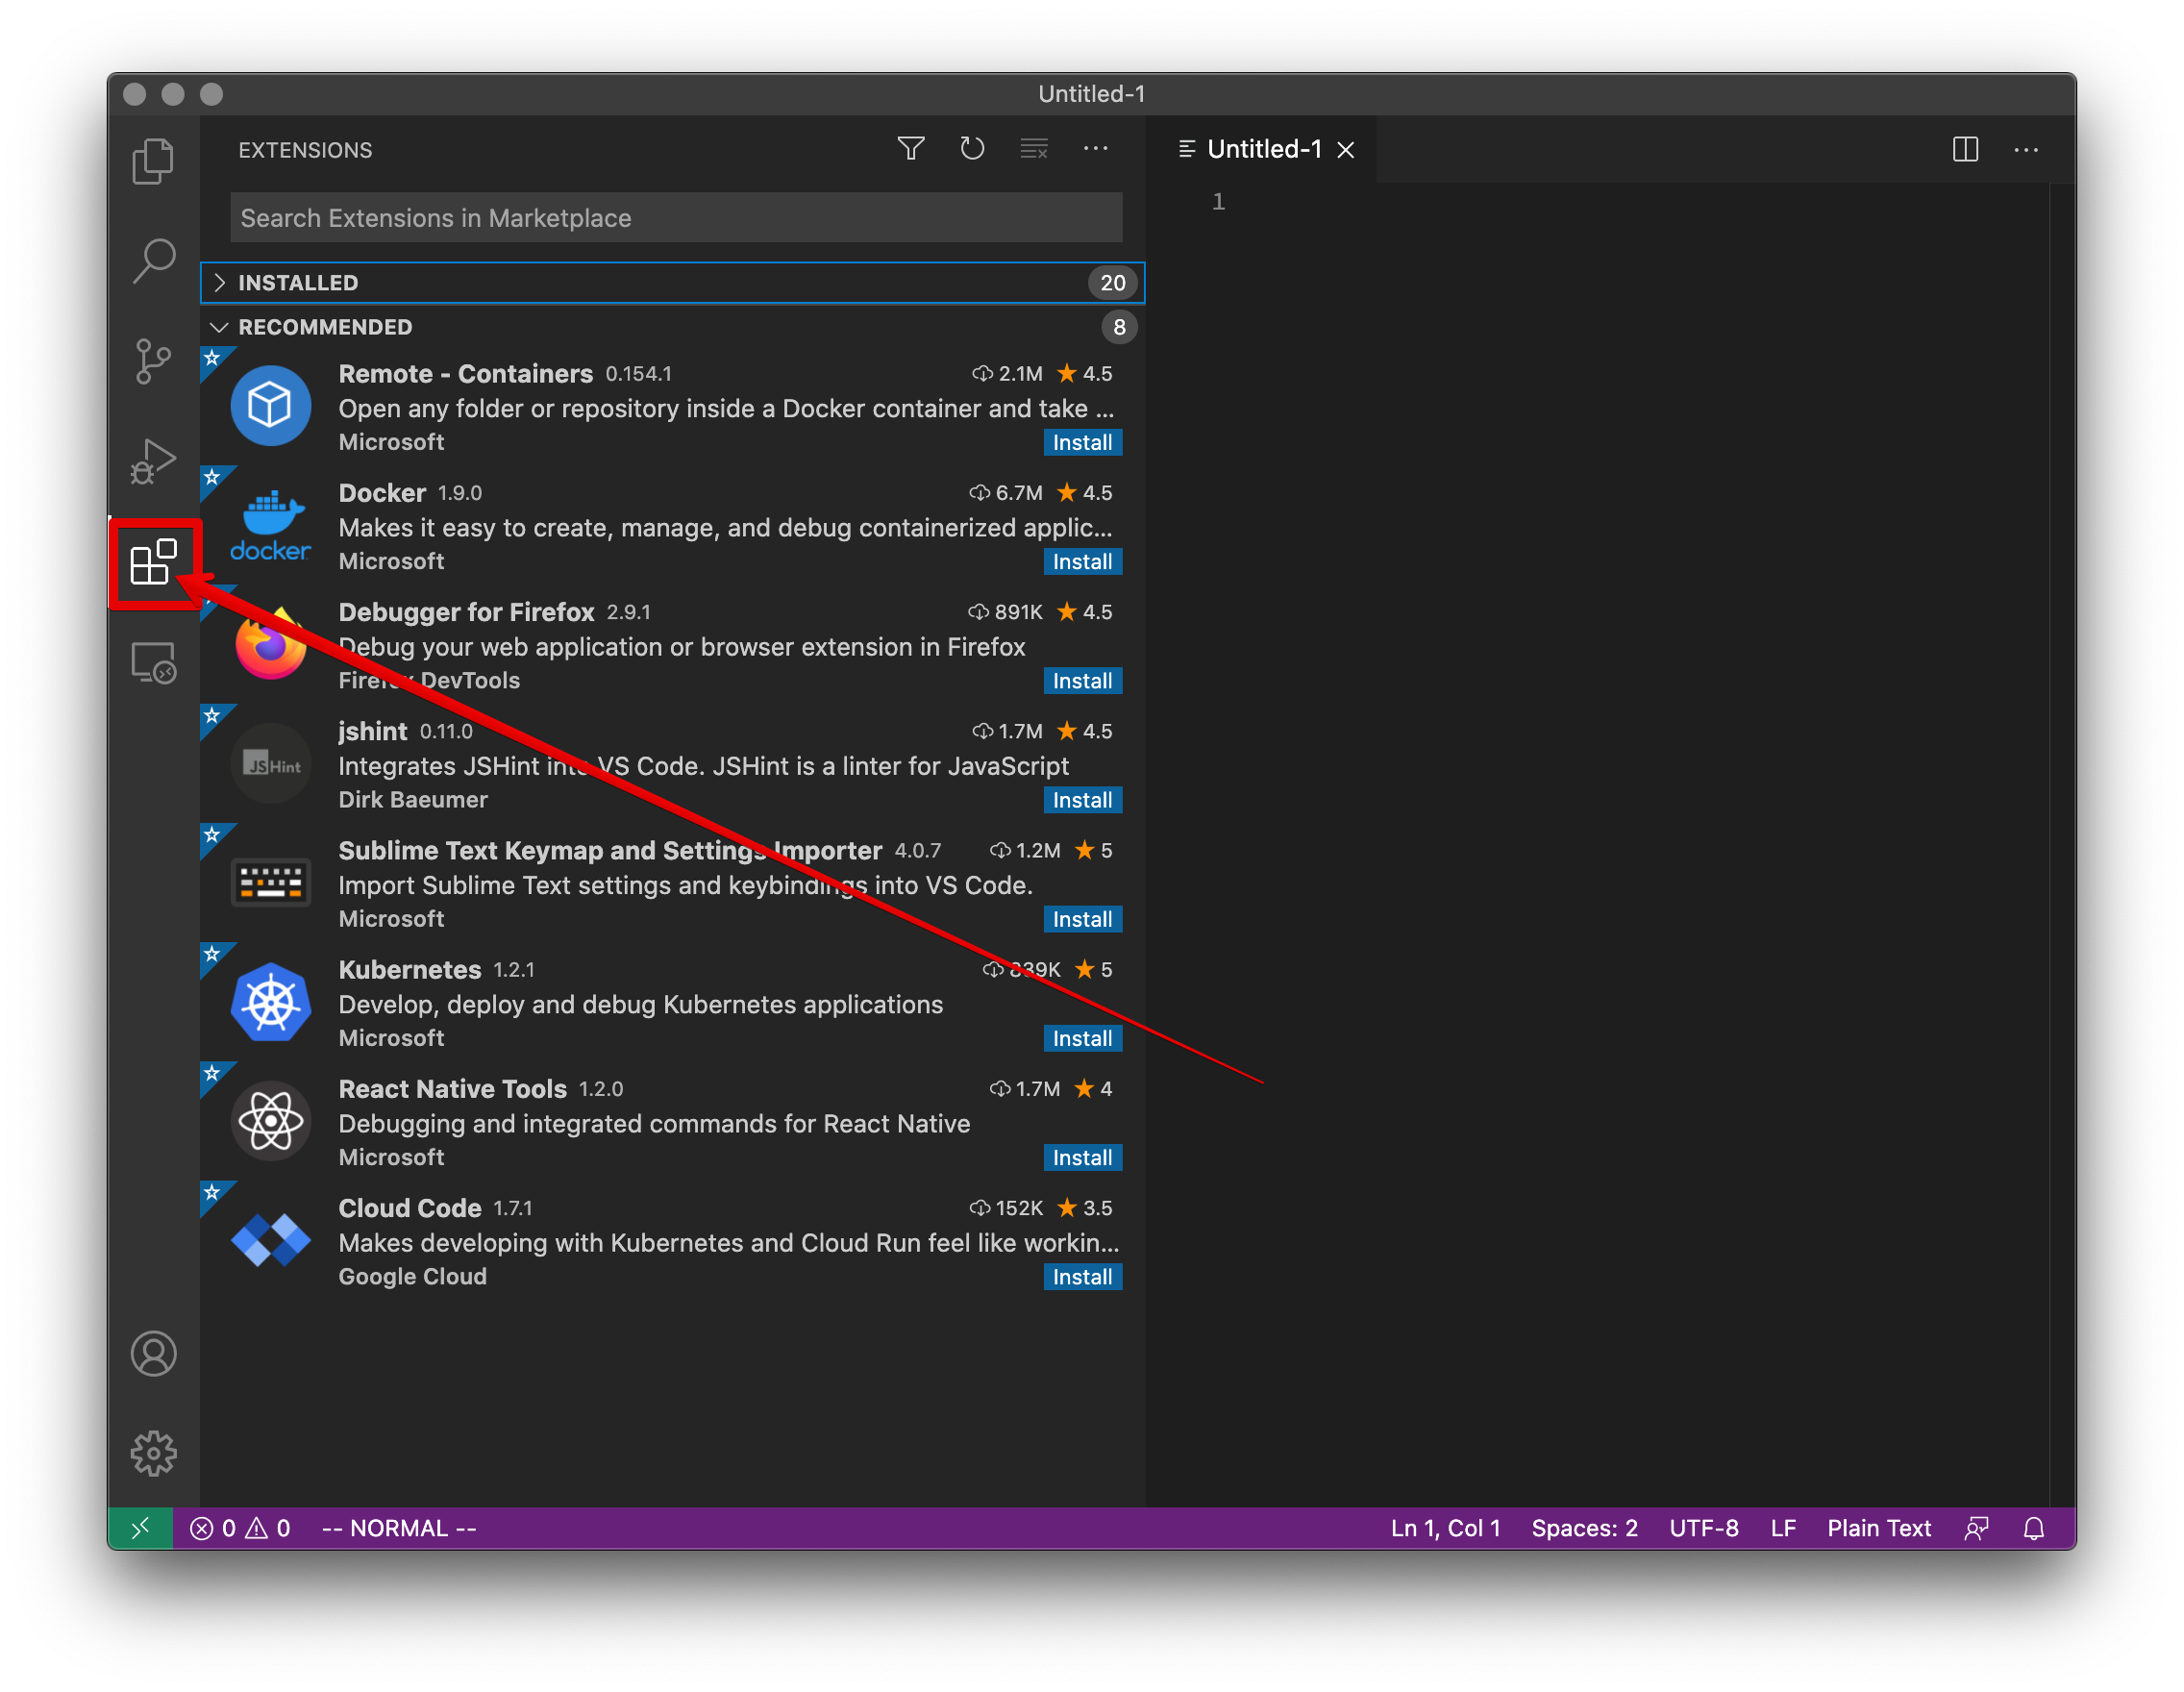
\includegraphics[width=1.0\maxwidth]{./images/01-createDevEnv/01_03vscodeExtension.png}%
\reviewimagecaption{VSCodeの拡張機能}
\label{image:01-createDevEnv:01_03vscodeExtension}
\end{reviewimage}

ここの検索窓に拡張機能の名前、キーワードを入力して検索します。

\subsubsection*{Debugger for Chrome}
\keeplastskip{
  \label{sec:1-2-2-1}
  \par\nobreak
}

デバッグの際に、PCにインストールされているChromeを自動で起動してくれます。
ChromeのDevToolsは、非常に強力です。また、ChromeにもReact、Redux用の拡張機能を追加すると
更に便利になります。

\begin{reviewimage}[H]%%01_06vscodeExtension_debuggerForChrome
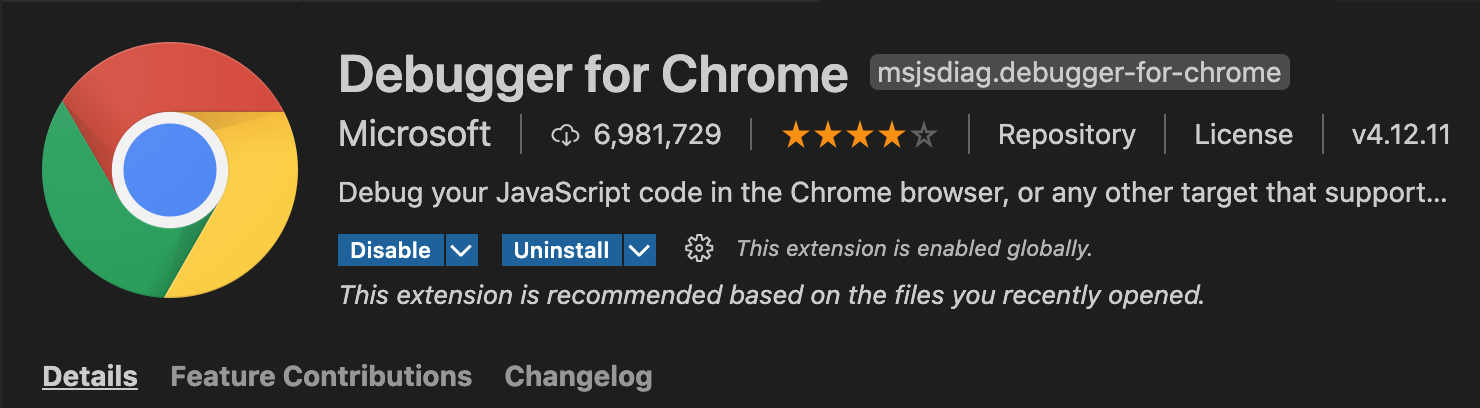
\includegraphics[width=1.0\maxwidth]{./images/01-createDevEnv/01_06vscodeExtension_debuggerForChrome.png}%
\reviewimagecaption{Beautify}
\label{image:01-createDevEnv:01_06vscodeExtension_debuggerForChrome}
\end{reviewimage}

\subsection{Eslint}
\keeplastskip{
  \label{sec:1-2-3}
  \par\nobreak
}

コード記法の間違いを指摘・修正してくれます。

\begin{reviewimage}[H]%%01_07vscodeExtension_eslint
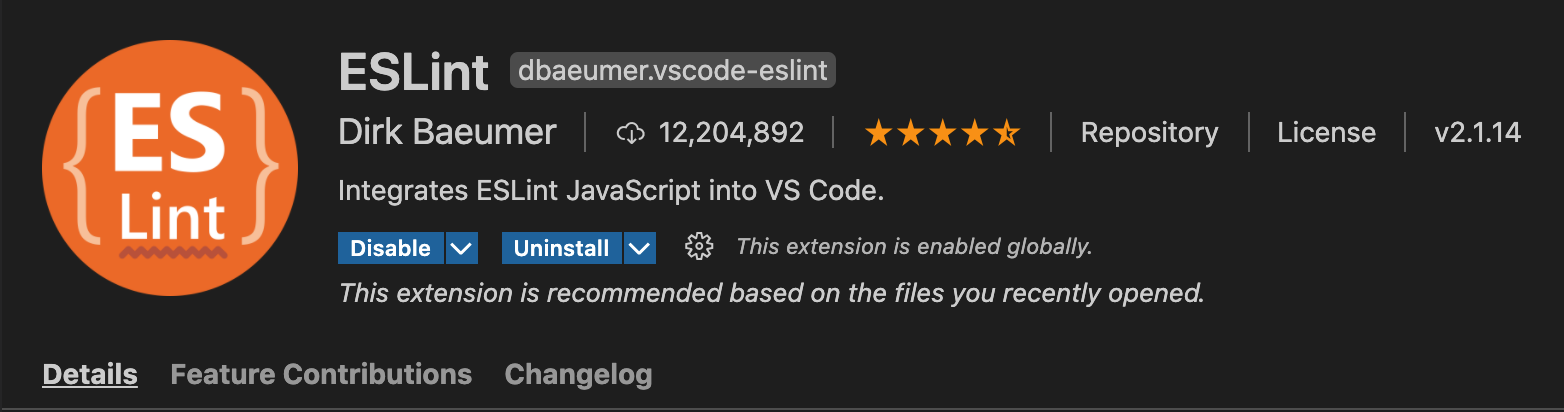
\includegraphics[width=1.0\maxwidth]{./images/01-createDevEnv/01_07vscodeExtension_eslint.png}%
\reviewimagecaption{Beautify}
\label{image:01-createDevEnv:01_07vscodeExtension_eslint}
\end{reviewimage}

\subsection{Prettier}
\keeplastskip{
  \label{sec:1-2-4}
  \par\nobreak
}

Eslintと同じように、コード記法の間違いの指摘・修正やコードフォーマットを行います。Eslintを合わせて使うと最強です。

\begin{reviewimage}[H]%%01_08vscodeExtension_prettier
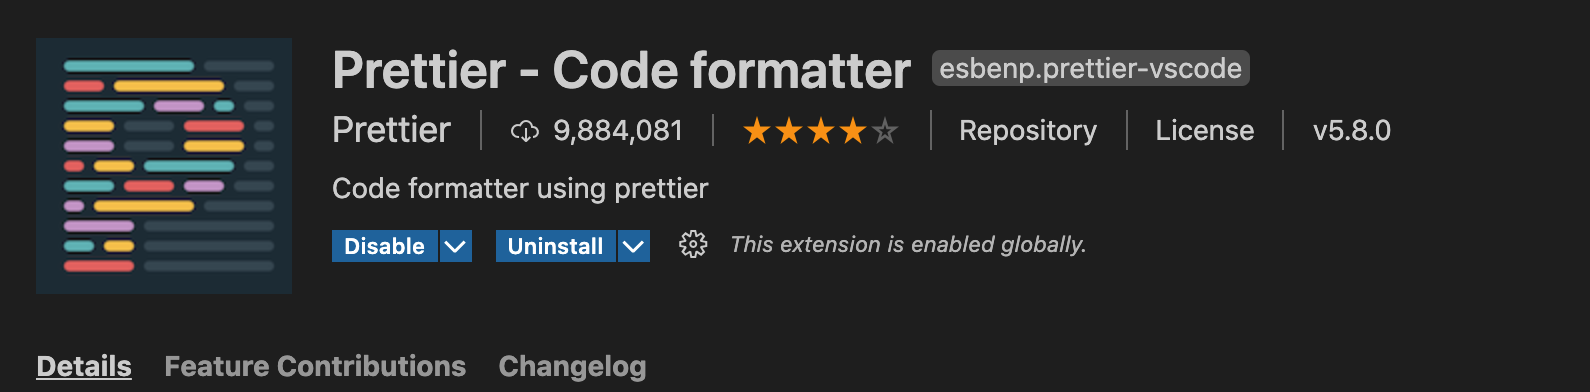
\includegraphics[width=1.0\maxwidth]{./images/01-createDevEnv/01_08vscodeExtension_prettier.png}%
\reviewimagecaption{Beautify}
\label{image:01-createDevEnv:01_08vscodeExtension_prettier}
\end{reviewimage}

\section{Google Chrome + 拡張機能}
\keeplastskip{
  \label{sec:1-3}
  \label{sec-chrome}
  \par\nobreak
}

ご存じGoogle社が提供するブラウザです。

PCへインストールされていない方は、\\[0pt]

\subsection{Google Chromeのインストール}
\keeplastskip{
  \label{sec:1-3-1}
  \par\nobreak
}

Google Chrome:\url{https://www.google.com/intl/ja/chrome/}

\begin{reviewimage}[H]%%01_09googleChrome
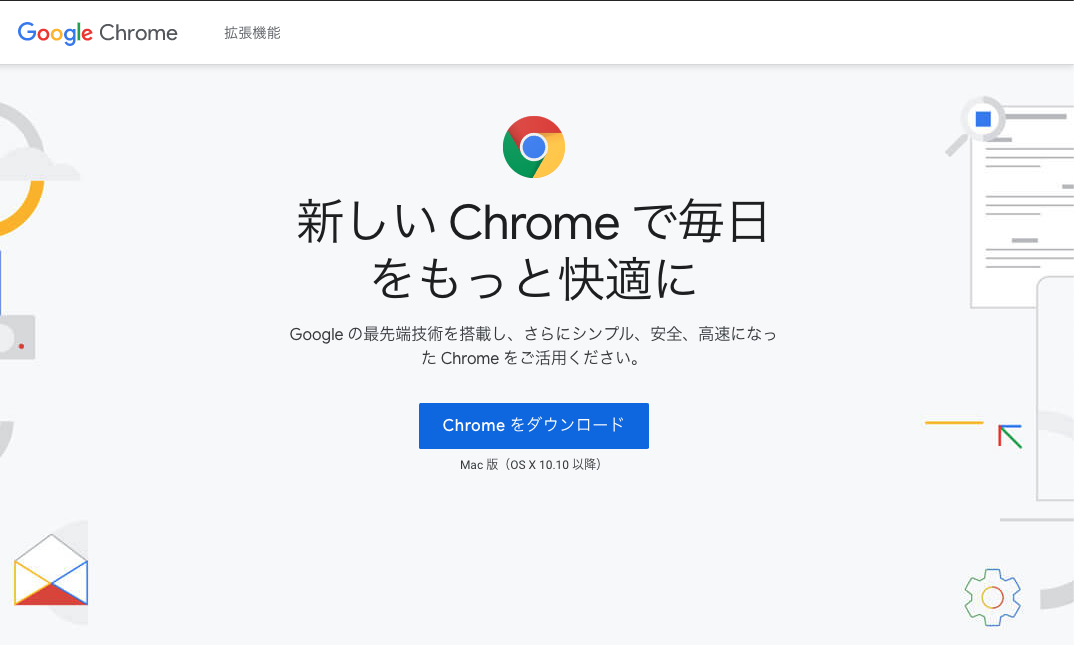
\includegraphics[width=1.0\maxwidth]{./images/01-createDevEnv/01_09googleChrome.png}%
\reviewimagecaption{Google Chrome}
\label{image:01-createDevEnv:01_09googleChrome}
\end{reviewimage}

\subsubsection*{Google Chromeの拡張機能}
\keeplastskip{
  \label{sec:1-3-1-1}
  \par\nobreak
}

こちらも、VSCodeと同様に拡張機能を追加することで、さらに便利に使うことができます。

React、Reduxの開発では、以下の拡張機能は必須と言っても良いほどです。

\vspace*{\baselineskip}

拡張機能のインストールは、下記のChrome Web storeで検索してください。

\vspace*{\baselineskip}

Chrome Web store:\url{https://chrome.google.com/webstore/category/extensions?hl=ja}

\begin{reviewimage}[H]%%01_13chromeWebstore
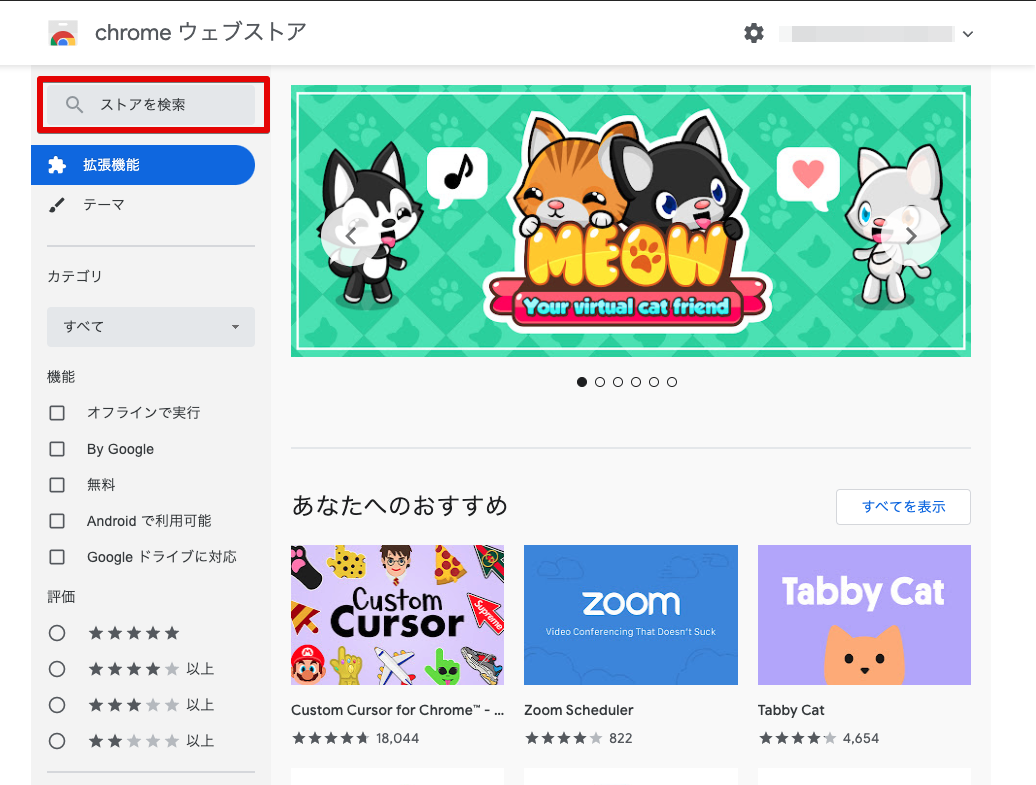
\includegraphics[width=1.0\maxwidth]{./images/01-createDevEnv/01_13chromeWebstore.png}%
\reviewimagecaption{Chrome Web store}
\label{image:01-createDevEnv:01_13chromeWebstore}
\end{reviewimage}

\clearpage


\subsubsection*{React Developer Tools}
\keeplastskip{
  \label{sec:1-3-1-2}
  \par\nobreak
}

Reactを使用して作成したページは、最終的にはページ出力用JavaScriptに変換され、ブラウザで表示されるときにはHTMLとして出力されます。
この拡張機能を使うと、Google ChromeのDevToolsにComponentsタブが作成され、Props、Stateを確認できます。

\begin{reviewimage}[H]%%01_10chromeExtReactDevTools
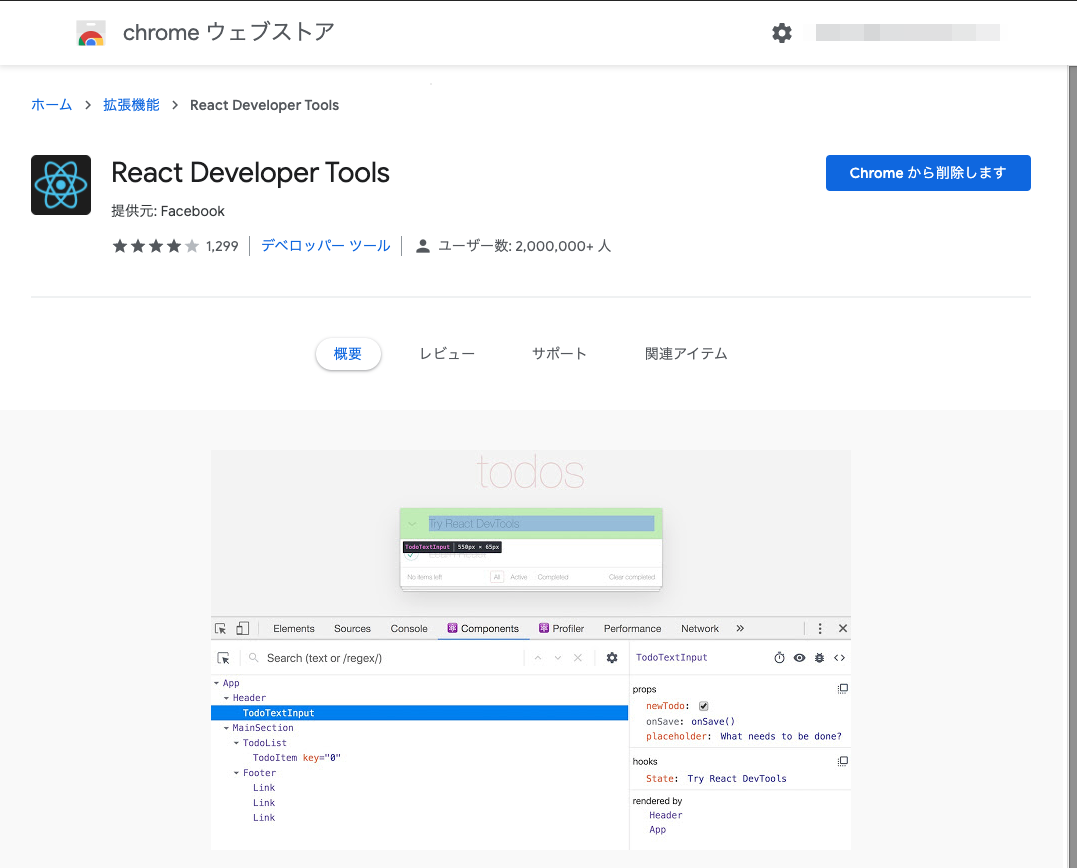
\includegraphics[width=1.0\maxwidth]{./images/01-createDevEnv/01_10chromeExtReactDevTools.png}%
\reviewimagecaption{React Developer Tools}
\label{image:01-createDevEnv:01_10chromeExtReactDevTools}
\end{reviewimage}
\begin{reviewimage}[H]%%01_12chromeExtReactDevTools01
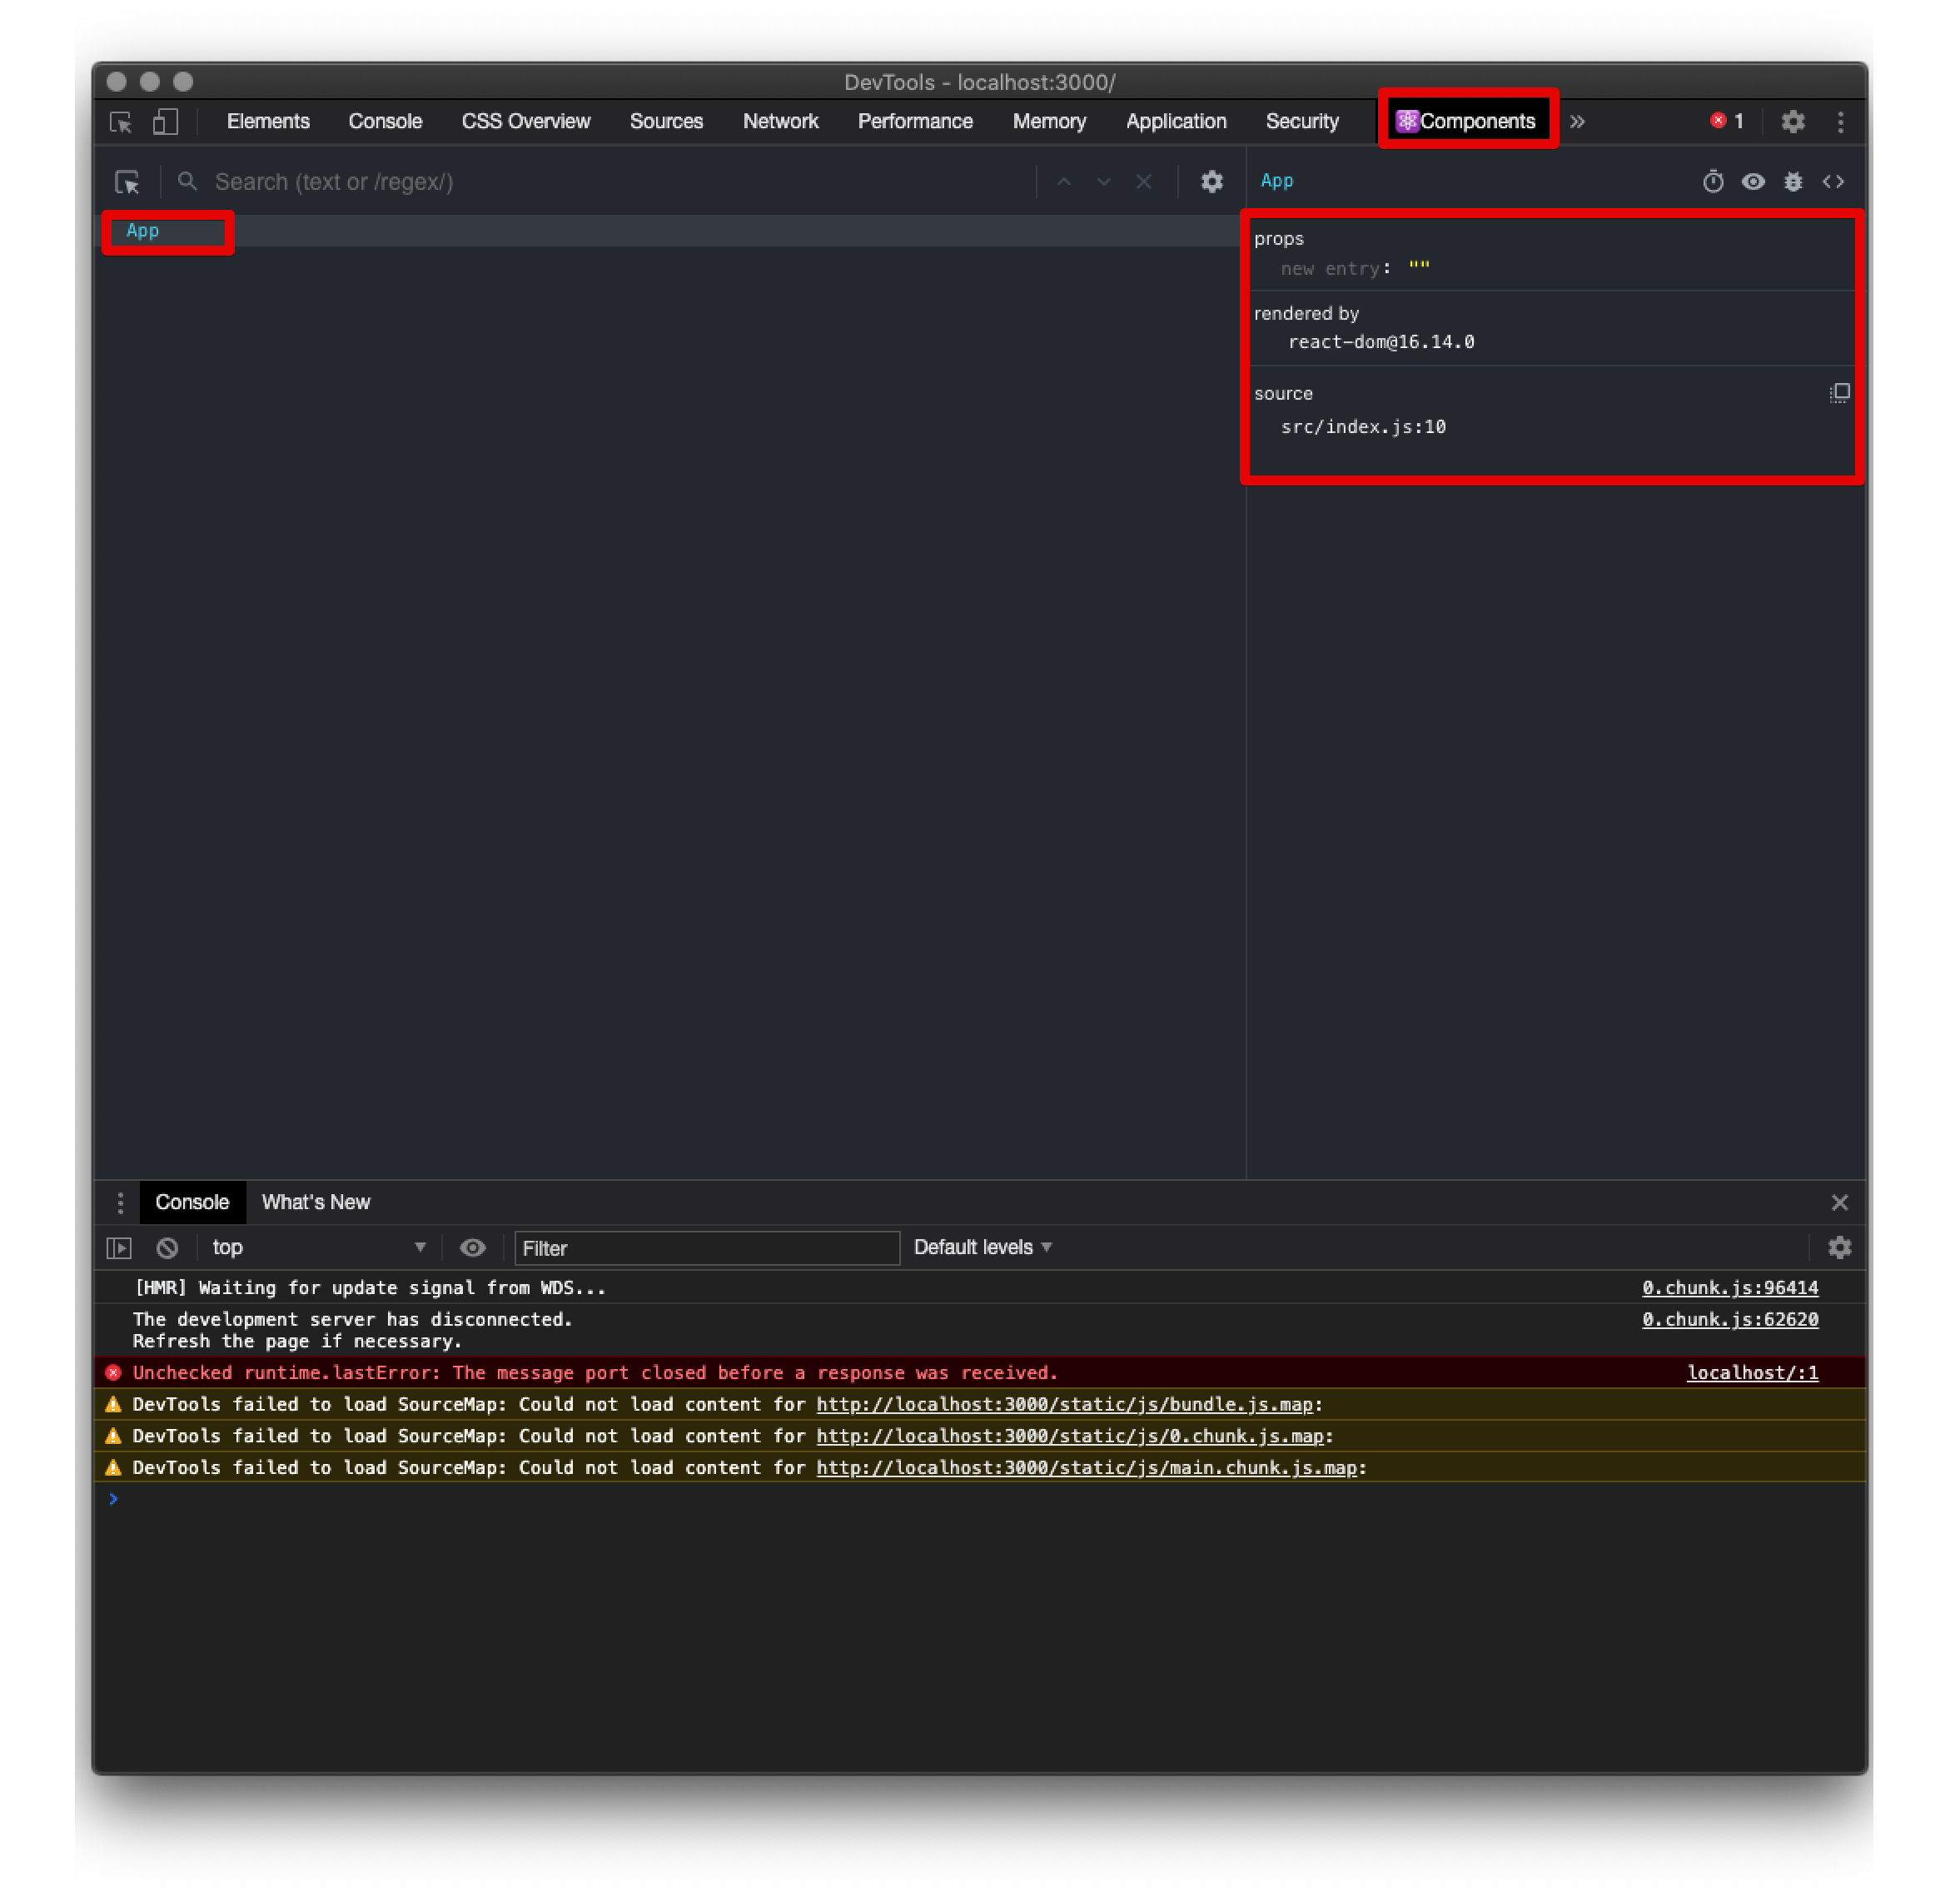
\includegraphics[width=1.0\maxwidth]{./images/01-createDevEnv/01_12chromeExtReactDevTools01.png}%
\reviewimagecaption{React DevToolsでAppを表示}
\label{image:01-createDevEnv:01_12chromeExtReactDevTools01}
\end{reviewimage}

\clearpage


\subsubsection*{Redux DevTools}
\keeplastskip{
  \label{sec:1-3-1-3}
  \par\nobreak
}

のちほど、Reduxの章であらためて説明しますが、「タイムトラベルデバッグ(実行されたアクションをさかのぼる)」が簡単にできます。
また、実行されたアクション、変更されたStateが「新」「旧」とあり、どの部分が変更されたのかも確かめるのも簡単です。

\begin{reviewimage}[H]%%01_11chromeExtReduxDevTools
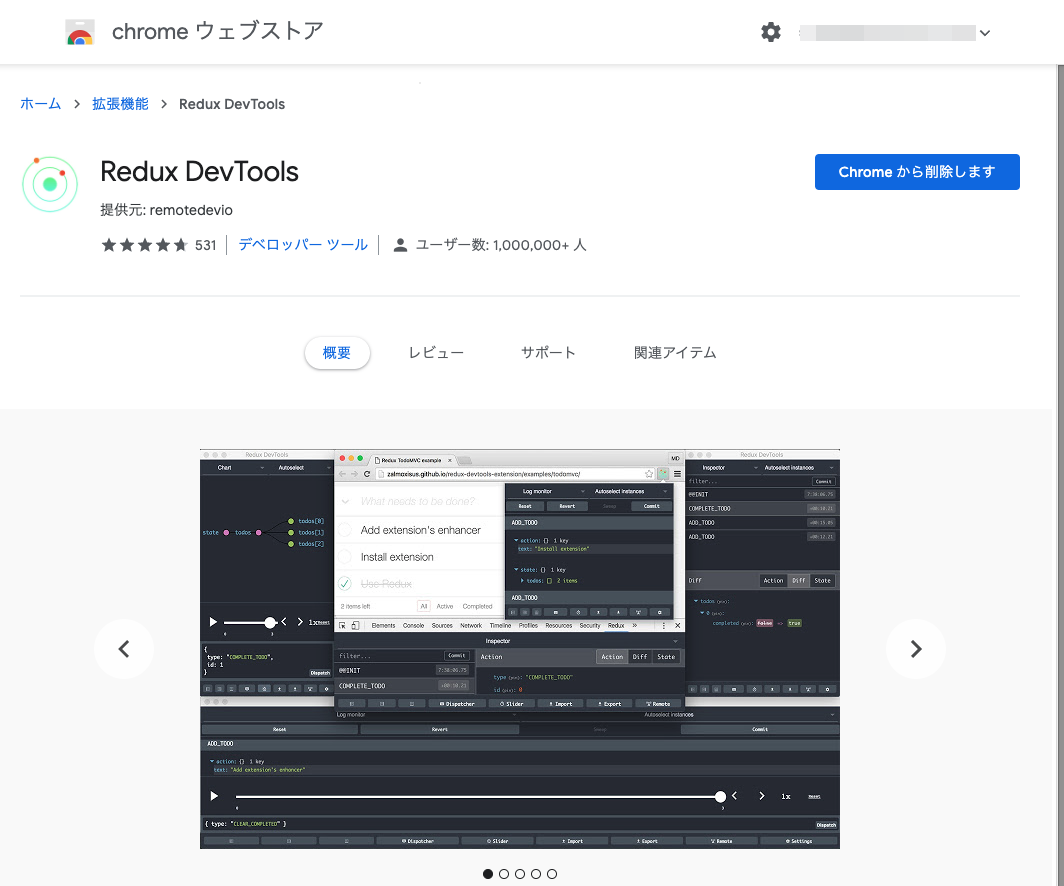
\includegraphics[width=1.0\maxwidth]{./images/01-createDevEnv/01_11chromeExtReduxDevTools.png}%
\reviewimagecaption{React DevloperTools拡張機能}
\label{image:01-createDevEnv:01_11chromeExtReduxDevTools}
\end{reviewimage}

\section{第1章のまとめ}
\keeplastskip{
  \label{sec:1-4}
  \label{sec-chap01review}
  \par\nobreak
}

React、Reduxの開発環境は、できましたでしょうか?

\begin{starteritemize}
\item nvm
\item node
\item VSCode + 拡張機能
\item Google Chrome + 拡張機能
\end{starteritemize}

のインストールを完了してください。
